\documentclass[a4paper,justified,nobib]{tufte-handout}
% Layout: tufte-handout class (CTAN tufte-latex, sample-handout.tex).
% Build: tectonic IT457_Week1_MagicPocket_Brief.tex

\usepackage{booktabs}
\usepackage{tabularx}
\usepackage{array}
\usepackage{amssymb}
\usepackage{tikz}
\usetikzlibrary{arrows.meta, positioning}
\usepackage{xurl}
\urlstyle{same}

\title[Dropbox Magic Pocket, Week 1]{Dropbox's Magic Pocket: leaving Amazon S3 for an in-house blob store}
\author[IT457 Case Study]{IT457 Cloud Computing \textperiodcentered{} Case study, Week 1 \textperiodcentered{} 202611054, 202611032, 202611009}
\date{21 October 2026}

\DeclareRobustCommand{\cite}[1]{\textsuperscript{[#1]}}
\setcounter{secnumdepth}{0}
% Plain running head; the class default trips over newer LaTeX releases.
\fancypagestyle{plain}{\fancyhf{}}
\fancyhf{}
\fancyhead[R]{\textsc{dropbox magic pocket \textperiodcentered{} week 1}\quad\thepage}

\begin{document}
\maketitle

\begin{abstract}
\noindent Between 2013 and 2016 Dropbox moved more than 90\% of roughly 600\,PB of user files
off Amazon S3 into Magic Pocket, a storage system it designed, wrote and runs in leased
co-location space. Below are the points that matter for the case, followed by the sources we found.
\end{abstract}

\section{Why leave S3}

\newthought{From its first year} Dropbox kept metadata and web servers in its own data centres
and only the file contents on S3.\cite{1} By 2015 those contents had grown to about 500\,PB,
twelve times the 40\,PB of 2012.\cite{1} The workload was narrow: immutable blocks of up to
4\,MB, written once and mostly read while fresh. Over 40\% of reads touch data from the last
day and over 90\% data from the last year.\cite{4} A general-purpose object store charges for
flexibility that such a workload never uses, and because storage is most of Dropbox's cost of
revenue, the S3 bill effectively set the company's gross margin. At this size, the fixed cost
of a dedicated team and custom hardware could be paid back, and owning the stack also meant
control over disk format, erasure code and repair policy.

\section{How the move was run}

\begin{margintable}
\footnotesize
\begin{tabular}{@{}l@{\quad}l@{}}
\toprule
Summer 2013 & project starts \\
Aug 2014 & dark launch, dual writes \\
27 Feb 2015 & serves users \\
30 Apr 2015 & BASE Jump bulk copy \\
7 Oct 2015 & 90\% in-house \\
Q4 2016 & S3 copies retired \\
\bottomrule
\end{tabular}
\caption{Migration timeline.\cite{1,8}}
\end{margintable}
After a dark launch in August 2014, every write went to both systems and spare copies stayed
on S3 for six months. The bulk copy, called BASE Jump, peaked above half a terabit per
second, and the 90\% mark was reached on 7 October 2015, three weeks early and with no data
lost.\cite{1} The duplicated data was not free: the S-1 notes higher storage cost until the
last S3 copies were retired in Q4 2016.\cite{8} Part way through, the disk-facing storage
engine was rewritten from Go in Rust, because Go's memory footprint was too large for dense
storage servers.\cite{11}

\section{Architecture}

\begin{figure}
\centering
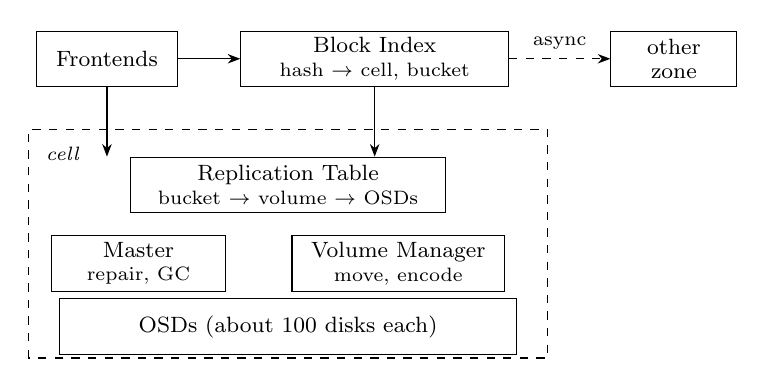
\begin{tikzpicture}[x=1mm, y=1mm, font=\footnotesize,
  b/.style={draw, align=center, inner sep=2pt, minimum height=7mm},
  >={Stealth[length=1.6mm]}]
  \node[b, minimum width=18mm] (fe) at (0,24) {Frontends};
  \node[b, minimum width=34mm] (bi) at (34,24) {Block Index\\[-1pt]\scriptsize hash $\to$ cell, bucket};
  \node[b, minimum width=16mm] (oz) at (72,24) {other\\[-1pt]zone};
  \draw[dashed] (-10,-14) rectangle (56,15);
  \node[anchor=north west, font=\scriptsize\itshape] at (-9,14) {cell};
  \node[b, minimum width=40mm] (rt) at (23,8) {Replication Table\\[-1pt]\scriptsize bucket $\to$ volume $\to$ OSDs};
  \node[b, minimum width=22mm] (ms) at (4,-2) {Master\\[-1pt]\scriptsize repair, GC};
  \node[b, minimum width=27mm] (vm) at (37,-2) {Volume Manager\\[-1pt]\scriptsize move, encode};
  \node[b, minimum width=58mm] (os) at (23,-10) {OSDs (about 100 disks each)};
  \draw[->] (fe) -- (bi);
  \draw[->] (fe.south) -- (fe.south |- rt.north);
  \draw[->] (bi.south) -- (bi.south |- rt.north);
  \draw[->, dashed] (bi) -- node[above, font=\scriptsize] {async} (oz);
\end{tikzpicture}
\caption{Magic Pocket within one zone, simplified from Cowling.\cite{2} A cell holds roughly
50--100\,PB; one Master per cell is what limits its size. Every block is copied to a second of
the three US zones within about a second.}
\end{figure}

\newthought{Files are split} into blocks of at most 4\,MB, each named by its SHA-256 hash.
Blocks are packed into 1\,GB \emph{buckets}, and buckets into \emph{volumes} that sit on a set
of storage servers (OSDs). Two MySQL tables hold all placement state: the sharded Block Index
maps a hash to its cell and bucket, and the Replication Table maps a bucket to its volume and
disks.\cite{2} The OSDs themselves are kept simple. A Master per cell schedules repair and
garbage collection but stays off the read and write path, and Volume Managers do the heavy
copying and encoding.

New writes go to volumes replicated four ways. When a volume fills it is closed and
erasure-coded with an LRC-(12,2,2) code: about 1.33$\times$ overhead against 1.5$\times$ for
Reed--Solomon (6,3), while still surviving any three failures in a group.\cite{10,12}

\section{Durability as a process}

\marginnote{The six verifiers:\cite{3} a Storage Watcher re-reads 1\% of new blocks after a
minute, hour, day, week and month; a Metadata Scanner checks about a million blocks a
second; a Disk Scrubber reads every disk each one to two weeks; three more checkers make
sure nothing is deleted without a log entry. Durability claims differ by source: 27 nines
in the model, 12 on the blog,\cite{1} 11 in the S-1.\cite{8}}
Cowling's ``Pocket Watch'' post is the least cited and most useful source here.\cite{3}
A Markov model of disk failure and repair gives 27 nines, but models leave out software bugs
and operator mistakes, so Dropbox runs six independent verifiers, and more than half of all
disk and database load is this self-checking. At today's scale there are hundreds of hardware
failures a day and about four 1--2\,GB extents are repaired every second, within a 48-hour
SLA.\cite{10}

\section{Lowering the cost per byte, 2016--2026}

\newthought{The design} has kept changing. In 2019 a cold tier split old blocks in two, stored
the halves in two regions and their XOR in a third. That cut the replication factor from
2$\times$ to 1.5$\times$, saving 25\% of disk, and tail latency actually improved because reads
go to all three regions and take the first two answers.\cite{4} Dropbox had first tried a
single erasure code across regions and dropped it after nine months. From 2018 it moved to
shingled (SMR) drives written as raw zones with no filesystem, about 20\% more capacity per
drive for roughly the same price;\cite{5} by 2025 over 99\% of the fleet was SMR, on drives of
up to 32\,TB.\cite{6} Between the fourth and sixth server generations, each exabyte needed
five fewer megawatts and a third of the rack space.\cite{5} The newest change, in April 2026,
fixed fragmentation left by a new on-the-fly erasure coder, with some volumes under 5\% full,
using a packing-based compaction step.\cite{7}

\section{What it saved, and what it did not}

\begin{margintable}
\centering
\footnotesize
\begin{tabular}{@{}lrrr@{}}
\toprule
\$M & 2015 & 2016 & 2017 \\
\midrule
Revenue & 604 & 845 & 1{,}107 \\
Cost of rev. & 407 & 391 & 369 \\
Gross margin & 33\% & 54\% & 67\% \\
Capex & 79 & 115 & 25 \\
\bottomrule
\end{tabular}
\caption{From Dropbox's S-1.\cite{8} Revenue nearly doubled while cost of revenue fell.}
\end{margintable}

\newthought{The S-1} is the only audited source.\cite{8} It credits ``Infrastructure
Optimization'' with cutting cost of revenue by \$39.5M in 2016 (\$92.5M less paid to the
``third-party datacenter service provider'', offset by \$53.0M of depreciation and facility
costs) and by a further \$35.1M in 2017. The often-quoted \$74.6M is the sum of the two; the
filing never states it. The same filing lists co-location sites in California, Texas and
Virginia.

Three caveats keep the story honest. First, Dropbox never left AWS: the remaining data and
some services stayed there, and from 2016 European business files have been stored on AWS in
Germany.\cite{1,13} Second, savings in cost of revenue leave out capital spending, about
\$219M over 2015--2017, and capital leases; Quinn uses exactly this to dispute a16z's claim
that owned infrastructure costs a third to a half of cloud.\cite{14,15} The FY2024 10-K still
shows \$92.7M a year of finance-lease cost for infrastructure.\cite{9} Third, the case
depends on one large, predictable, storage-heavy workload, which most companies do not have.

\section{Plan for Weeks 2 and 3}

We follow the cost and repatriation exercise. We will price a 1\,EB, mostly cold blob
workload on S3 and one other provider using their calculators, then build a bottom-up
on-premises estimate (SMR drives, servers, power at about 0.3--0.5\,W per TB,\cite{5}
co-location and staff). On a small test cluster we will also measure the storage overhead of
three-way replication, erasure coding and the 2+1 XOR scheme.

% ======================= SOURCES =======================
\section{Sources found}



\begin{fullwidth}
\footnotesize
\noindent Tags: \textsc{p} primary (Dropbox or its filings), \textsc{c} talk or interview by
Dropbox engineers, \textsc{a} academic, \textsc{s} secondary or commentary, \textsc{v} vendor.

\begin{list}{}{\setlength{\leftmargin}{2.2em}\setlength{\labelwidth}{1.8em}\setlength{\labelsep}{0.4em}\setlength{\itemsep}{1.5pt}\setlength{\parsep}{0pt}}
\item[{[1]}] {\scshape\MakeLowercase{P}}\enspace A.~Gupta, ``Scaling to exabytes and beyond,'' \textit{dropbox.tech}, 14 Mar 2016. \textit{Used for:} Timeline from 2013 to Oct 2015, 500\,PB scale, durability and availability targets, hybrid set-up. \url{https://dropbox.tech/infrastructure/magic-pocket-infrastructure}
\item[{[2]}] {\scshape\MakeLowercase{P}}\enspace J.~Cowling, ``Inside the Magic Pocket,'' \textit{dropbox.tech}, 6 May 2016. \textit{Used for:} Blocks, buckets, volumes and cells; the two MySQL tables; roles of Master, Volume Manager and OSD. \url{https://dropbox.tech/infrastructure/inside-the-magic-pocket}
\item[{[3]}] {\scshape\MakeLowercase{P}}\enspace J.~Cowling, ``Pocket watch: verifying exabytes of data,'' \textit{dropbox.tech}, 6 Jul 2016. \textit{Used for:} 27-nines model; the six verifiers; more than half of disk load spent on checking. \url{https://dropbox.tech/infrastructure/pocket-watch}
\item[{[4]}] {\scshape\MakeLowercase{P}}\enspace P.~Le, ``How we optimized Magic Pocket for cold storage,'' \textit{dropbox.tech}, 6 May 2019. \textit{Used for:} 2+1 XOR cold tier, 25\% saving, latency percentiles, read-age statistics, abandoned designs. \url{https://dropbox.tech/infrastructure/how-we-optimized-magic-pocket-for-cold-storage}
\item[{[5]}] {\scshape\MakeLowercase{P}}\enspace E.~Shobe, ``After four years of SMR storage,'' \textit{dropbox.tech}, 8 Mar 2023. \textit{Used for:} SMR without a filesystem; watts per TB; power and space per EB by server generation. \url{https://dropbox.tech/infrastructure/four-years-of-smr-storage-what-we-love-and-whats-next}
\item[{[6]}] {\scshape\MakeLowercase{P}}\enspace E.~Shobe and J.~Mednick, ``Seventh-generation server hardware,'' \textit{dropbox.tech}, 2 Jul 2025. \textit{Used for:} 32\,TB SMR drives, SMR share of fleet, rack power and storage bandwidth targets. \url{https://dropbox.tech/infrastructure/seventh-generation-server-hardware}
\item[{[7]}] {\scshape\MakeLowercase{P}}\enspace F.~Agriel, ``Improving storage efficiency in Magic Pocket,'' \textit{dropbox.tech}, 2 Apr 2026. \textit{Used for:} Fragmentation incident and the L1/L2/L3 compaction strategies. \url{https://dropbox.tech/infrastructure/improving-storage-efficiency-in-magic-pocket-our-immutable-blob-store}
\item[{[8]}] {\scshape\MakeLowercase{P}}\enspace Dropbox Inc., Form S-1, SEC EDGAR, Feb 2018. \textit{Used for:} Cost of revenue, gross margin, capex, capital leases, data centre locations, remaining AWS use, risk factors. \url{https://www.sec.gov/Archives/edgar/data/0001467623/000119312518055809/d451946ds1.htm}
\item[{[9]}] {\scshape\MakeLowercase{P}}\enspace Dropbox Inc., Form 10-K for FY2024, SEC EDGAR, Feb 2025. \textit{Used for:} Finance-lease cost of infrastructure in 2024. \url{https://www.sec.gov/Archives/edgar/data/1467623/000146762325000011/dbx-20241231.htm}
\item[{[10]}] {\scshape\MakeLowercase{C}}\enspace F.~Agriel, ``Magic Pocket: Dropbox's exabyte-scale blob storage system,'' QCon SF 2022; InfoQ write-up, 15 May 2023. \textit{Used for:} 600k+ drives, 4$\times$ replication then LRC-(12,2,2), repair rate and SLA, lessons. \url{https://www.infoq.com/articles/dropbox-magic-pocket-exabyte-storage/}
\item[{[11]}] {\scshape\MakeLowercase{C}}\enspace J.~Cowling, ``Dropbox's Magic Pocket,'' \textit{Software Engineering Daily} (podcast), 2016; C.~Metz, \textit{Wired}, Mar 2016. \textit{Used for:} Design reasoning from the lead engineer; the team and the Go to Rust rewrite. \url{https://softwareengineeringdaily.com/podcasts/dropboxs-magic-pocket-james-cowling/}
\item[{[12]}] {\scshape\MakeLowercase{A}}\enspace C.~Huang et al., ``Erasure coding in Windows Azure Storage,'' USENIX ATC 2012; S.~Muralidhar et al., ``f4: Facebook's warm BLOB storage system,'' OSDI 2014. \textit{Used for:} The LRC family behind Magic Pocket's code, and the f4 XOR design Dropbox considered for its cold tier.
\item[{[13]}] {\scshape\MakeLowercase{P/S}}\enspace Dropbox blog, ``Dropbox is growing in Europe,'' Feb 2016; \textit{Fortune}, 23 May 2016. \textit{Used for:} European business data placed on AWS in Germany. \url{https://fortune.com/2016/05/23/dropbox-germany}
\item[{[14]}] {\scshape\MakeLowercase{S}}\enspace S.~Wang and M.~Casado, ``The cost of cloud, a trillion dollar paradox,'' a16z, May 2021. \textit{Used for:} Dropbox as the leading repatriation example; the one-third-to-one-half rule. \url{https://a16z.com/the-cost-of-cloud-a-trillion-dollar-paradox/}
\item[{[15]}] {\scshape\MakeLowercase{S}}\enspace C.~Quinn, ``The trillion-dollar paradoxical arguments of a16z,'' \textit{Last Week in AWS}, 16 Jun 2021. \textit{Used for:} The counter-argument: capex outside cost of revenue, a single predictable workload. \url{https://www.lastweekinaws.com/blog/the-trillion-dollar-paradoxical-arguments-of-a16z}
\item[{[16]}] {\scshape\MakeLowercase{V}}\enspace Seagate, ``Powering AI at scale: Dropbox qualifies Seagate's Exos 32TB drives,'' 29 Sep 2025. \textit{Used for:} HAMR drives qualified in June 2025 without new racks; inputs for our cost model. \url{https://www.seagate.com/blog/powering-ai-at-scale/}
\end{list}

\vspace{2mm}
\noindent\textit{Corrections to our first draft.} SMR was first deployed in 2018, not 2020;
``500 million'' counts sign-ups, not active users; \$74.6M is a two-year sum we computed, not
a figure printed in the S-1, and not an annual saving.


\end{fullwidth}

\end{document}
